% !TEX root = mythesis.tex

%==============================================================================
\chapter{LHC and the ATLAS detector}
\label{sec:lhcandatlas}
%==============================================================================
The purpose of this chapter is to describe the machinery behind the production of the data. A brief overview of the Large Hadron Collider and a detailed description of the ATLAS detector is given. An introduction to the coordinate system, which is used by the ATLAS detector and the detailed explanation of all the sub-detector components of the detector is given in the last section of the chapter.

%------------------------------------------------------------------------------
\section{The Large Hadron Collider (LHC)}%
\label{sec:lhcandatlas:lhc}
%------------------------------------------------------------------------------
The Large Hadron Collider (LHC)~\cite{lhc} is a proton-proton collider situated at the Swiss-French border. The collider is built in a \SI{26.7}{\kilo\metre} circular tunnel which is approximately \SI{100}{\metre} underground. It is designed to collide protons at $\sqrt{s}$=\SI{13}{\tera\electronvolt}, which makes it the highest energy particle collider ever built. The high centre-of-mass energy is essential for the possible production of new exotic particles. The collider is designed to have high luminosity of particle collisions, $\SI{1e34}{\centi\metre^{-2}\sec^{-1}}$. The high luminosity means that rare events (with low cross-section) will occur at relatively high rates. The LHC was operational for two significant periods of time, called Run 1 and Run 2 respectively. Run 1 corresponds to the data collected from 2009 to 2013 at $\sqrt{s}=\SI{7}{\tera\electronvolt}$ and $\sqrt{s}=\SI{8}{\tera\electronvolt}$. Then it was shut down for two years. After that, the data collected from 2015 to 2018 at $\sqrt{s}=\SI{13}{\tera\electronvolt}$ corresponds to Run 2 phase. In this thesis, the data collected during Run 2 is used for the analysis.

To achieve such high energy, several accelerating machines are required. An overview of the main components of the accelerator complex is shown in Fig.\ \ref{fig:lhcandatlas:lhc}. Protons are first injected to the pre-accelerator, which includes linear accelerator \enquote{LINAC 2} where protons are accelerated to an energy of \SI{1.4}{\giga\electronvolt} and then injected to the Booster. The Booster also groups the protons in bunches of around \num{1e11} protons before injecting them into the Proton Synchrotron (PS). The PS accelerates the proton bunches up to an energy of \SI{25}{\giga\electronvolt} before injecting them into the Super Proton Synchroton (SPS). The SPS accelerates the protons up to an energy of \SI{450}{\giga\electronvolt}. After the proton bunches are injected into the LHC, where they are accelerated to a maximum energy of \SI{6.5}{\tera\electronvolt} per beam. After reaching this energy, protons are injected into two separate beam pipes. Protons in one of these pipes circulate clock-wise, while protons in the other beam pipe travel in the opposite direction. The LHC uses approximately \num{1300} dipole magnets to circulate the proton bunches around the ring about $\approx\num{11000}$ times a second, which generates a magnetic field of \SI{8.3}{\tesla}. The LHC also uses over \num{300} quadrupole magnets to keep the beams focused. The proton bunches become uncollimated over time. Therefore, another \num{5000} correcting magnets are used to keep the protons in bunches, and also to make orbital corrections as the protons circulate the LHC. With this setup, energies reached at the LHC during Run 2 resulted in center-of-mass energy of \SI{13}{\tera\electronvolt}, with an instantaneous luminosity of $\SI{1e34}{\centi\metre^{-2}\sec^{-1}}$. During Run 2, a total integrated luminosity of $\SI{156}{\femto\barn^{-1}}$ was delivered by the LHC, but $\SI{139}{\femto\barn^{-1}}$ was considered good enough for physics analyses.~\cite{lhc}~\cite{thesis:fletcher}

The proton beams are collided at different interaction points along the LHC ring, where the particle detectors are built to detect particles created during a collision. The four main experiments are shown in Fig.\ \ref{fig:lhcandatlas:lhc}. The two largest particle detectors, A Toroidal LHC ApparatuS (ATLAS)~\cite{atlas} and Compact Muon Solenoid (CMS)~\cite{cms} are general-purpose particle detectors, which have a wide-ranging physics searches which include both SM and BSM searches. Large Hadron Collider beauty (LHCb)\cite{lhcb} focuses on $b$-physics, which is a physics of rare decays of $b$-mesons and precise measurements of CP-violation in the SM. The fourth particle physics experiment, A Large Ion Collider Experiment (ALICE)~\cite{alice} is a heavy-ion experiment that is specifically designed to look at lead-lead ion and proton-lead ion collisions. It focuses on quark-gluon plasma, a primordial state of matter, which is thought to have existed in the early universe.


\begin{figure}[hbt!]
	\centering
	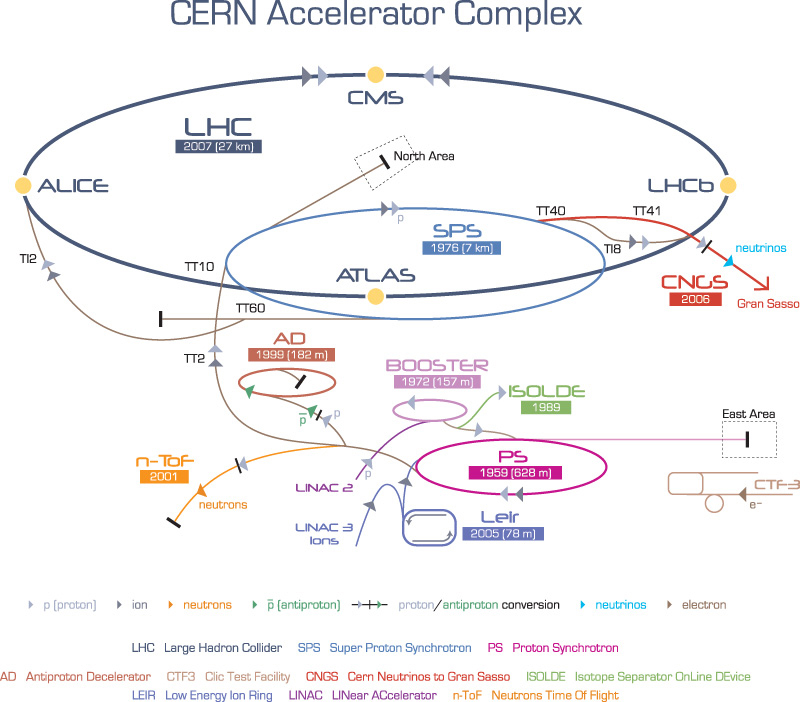
\includegraphics[width=0.9\linewidth]{lhc.jpg}
	\caption{A schematic showing the layout of the accelerator complex, which includes pre-accelerator and the LHC ring. The four interaction points are shown in yellow dots around the LHC ring where the four main experiments are built.~\cite{lhc_picture}}
	\label{fig:lhcandatlas:lhc}
\end{figure}



%------------------------------------------------------------------------------
\section{The ATLAS detector}%
\label{sec:lhcandatlas:atlas}
%------------------------------------------------------------------------------
The ATLAS detector (A Toroidal LHC ApparatuS)~\cite{atlas} is a multi-purpose particle detector which has dimensions of a total length of \SI{46}{\meter}, a height of \SI{25}{\meter} and a total weight of \SI{7000}{\tonne}. The ATLAS detector comprises of several layers of sub-detectors, where each is serving a specific function to detect one or more properties of the particles passing through them. These sub-detectors can be ordered into four categories: the inner detector (ID), the calorimeter system, the muon spectrometer and the magnet system. An overview of the detector is shown in Fig.\ \ref{fig:lhcandatlas:atlas}.~\cite{detector}
\begin{figure}[hbt!]
	\centering
	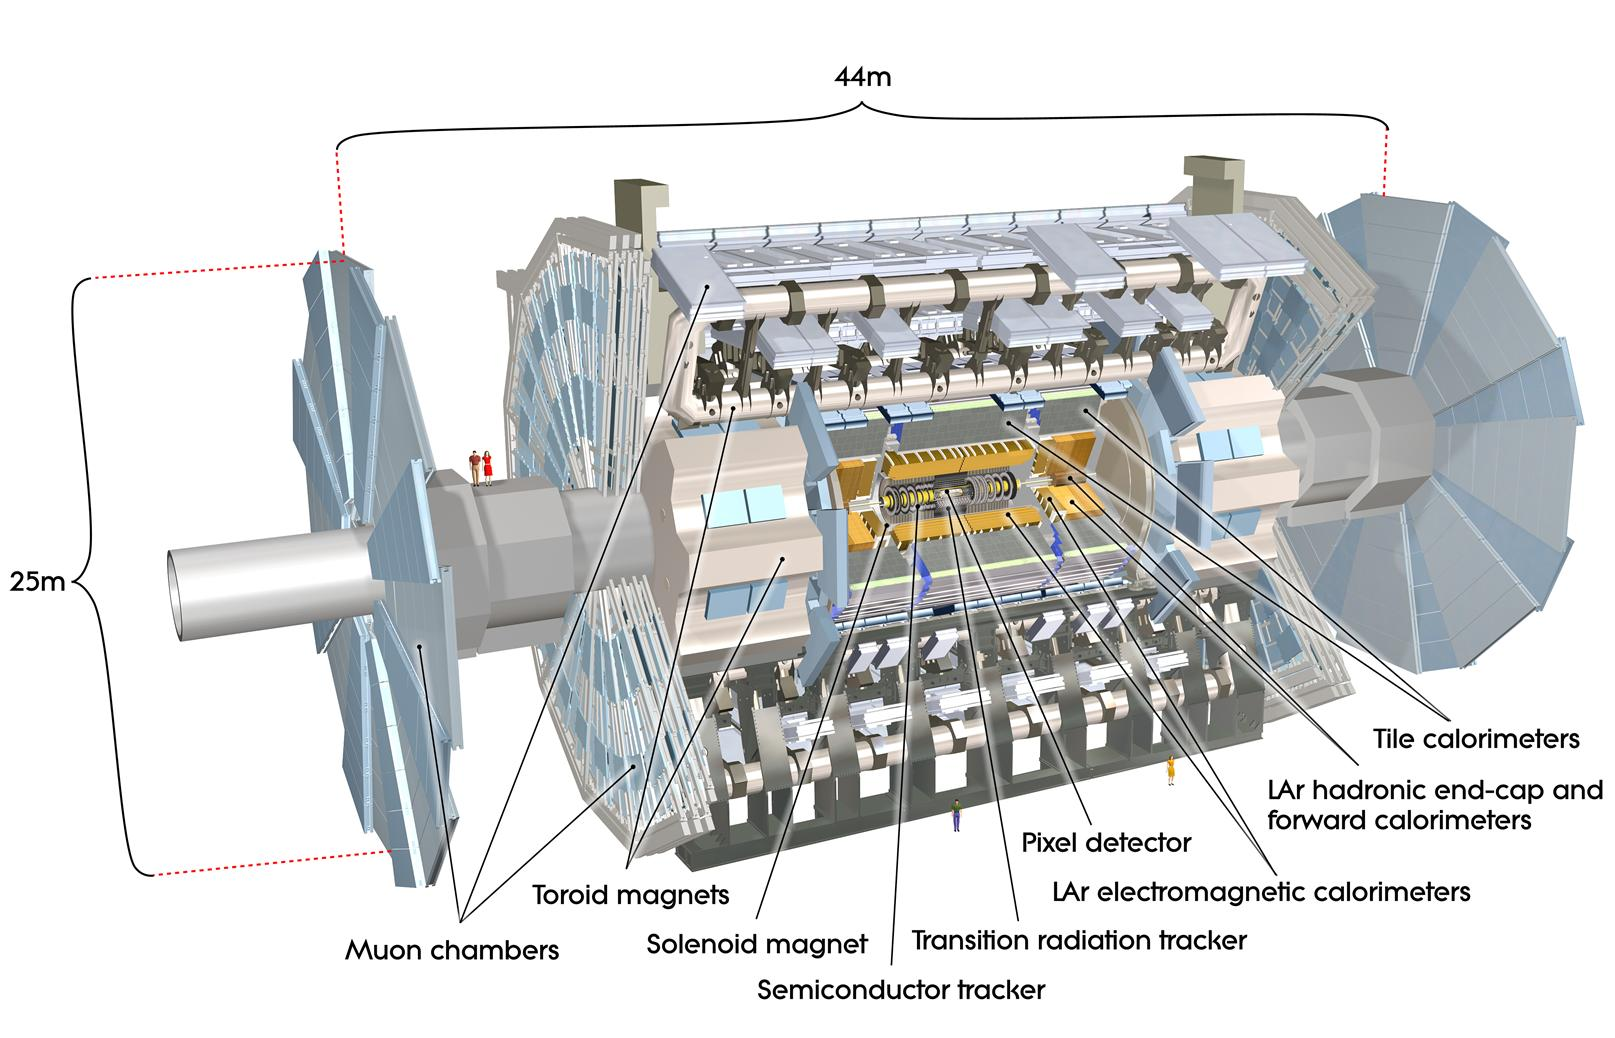
\includegraphics[width=0.9\linewidth]{detector.jpg}
	\caption{An overview of the ATLAS detector showing all the components of the detector.~\cite{detector}}
	\label{fig:lhcandatlas:atlas}
\end{figure}

%------------------------------------------------------------------------------
\subsection{Coordinate system and kinematic observables}%
\label{sec:lhcandatlas:atlas:observables}
%------------------------------------------------------------------------------
The ATLAS detector is based on a right-handed cartesian coordinate system with the x-axis pointing into the centre of the LHC collider ring, the y-axis denoting the vertical direction towards the surface and the z-axis along the LHC beam pipe.~\cite{detector} The ATLAS detector obeys a concentric cylindrical symmetry. Therefore, the spherical polar angles of $\theta$ and $\phi$ are used. The azimuthal angle ($\phi$) is measured around the beam axis in the z-axis direction, and the polar $\theta$ angle is measured as the angle from the beam axis. A schematic of the ATLAS coordinate system is shown in Fig.\ \ref{fig:lhcandatlas:atlas:observables}.
\begin{figure}[hbt!]
	\centering
	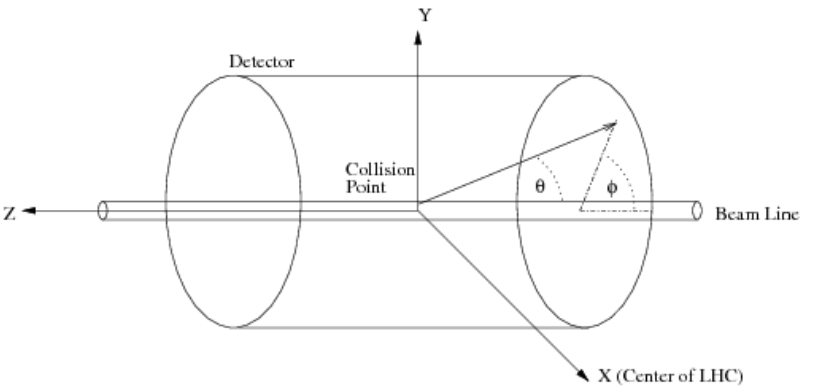
\includegraphics[width=0.7\linewidth]{coordinate.png}
	\caption{A schematic showing the coordinate system of the ATLAS detector.~\cite{atlas_coordinate}}
	\label{fig:lhcandatlas:atlas:observables}
\end{figure}
 
In the $pp$ collision at the LHC, partons are colliding with each other, where each of these partons carries a part of the proton momentum. Since the initial momentum is zero in the transverse plane, so it is convenient to define a quantity called transverse momentum:
\begin{equation}
	p_{\text{T}} = \sqrt{p_{\text{x}}^{\text{2}} + p_{\text{y}}^{\text{2}}} \,,
\end{equation}
where $p_{\text{x}}$ and $p_{\text{y}}$ are denoted as the momentum components in x and y directions, respectively. According to the conservation of momentum, the total momentum in the transverse plane should result in zero. Therefore, if the sum of all transverse momenta does not yield zero, the missing transverse momentum can be calulated as:
\begin{equation}
	p_{\text{T}}^{\text{miss}} = -\sum_{i}^{}p_{\text{T}i} \,,
\end{equation}
where $i$ is denoted as all the detected particles. It is used to find neutrinos since they pass through the detector undetected.

The centre-of-mass frame of the collision is usually Lorentz boosted in the z-axis, but the physics analyses need quantities that are invariant under a Lorentz boost. One such quantity which is invariant under a boost along the z-axis and gives information about the angular distribution of the particles, is rapidity $y$:
\begin{equation}
	y = \frac{1}{2}\ln(\frac{E+p_{\text{z}}}{E-p_{\text{z}}}) \,,	
\end{equation}
where $E$ is denoted is the energy of the particle and $p_{\text{z}}$ is represented as the momentum of the particle along the z-axis.

Pseudorapidity ($\eta$) is widely used instead of rapidity since the momentum of the partons along the z-axis is unknown, and it is defined as:
\begin{equation}
	\eta = -\ln{\tan(\frac{\theta}{2})} \,.
\end{equation}

It is also crucial to define a quantity that measures the distance between physics objects for the jet formation and to resolve the overlapped physics objects in the detector. The Lorentz invariant geometric variable $\Delta R$ is used for this, which is defined as:
\begin{equation}
	\Delta R = \sqrt{\Delta \eta^{\text{2}} + \Delta \phi^{\text{2}}} \,.
\end{equation}


%------------------------------------------------------------------------------
\subsection{Detector overview}%
\label{sec:lhcandatlas:atlas:components}
%------------------------------------------------------------------------------

%------------------------------------------------------------------------------
\subsubsection{Inner detector}%
\label{sec:lhcandatlas:atlas:inner}
%------------------------------------------------------------------------------
The Inner Detector (ID) is a cylindrical tracking detector which is placed close to the interaction point to reconstruct the primary vertex and measure the momentum of the tracks. The ID consists of the insertable B-layer (IBL), pixel detector, the semiconductor tracker (SCT) and the transition radiation tracker (TRT). The pixel detector is composed of the silicon pixel modules and the SCT is composed of the silicon microstrip sensors. They both are precision silicon tracking detectors and cover a pseudorapidity range of $|\eta|<2.5$. The TRT is a drift chamber made up of gas-filled straw tubes that includes a pseudorapidity range of $|\eta|<2.0$. The entire inner detector is kept in a magnetic field of \SI{2}{\tesla}, generated by the ATLAS solenoid magnet. The magnetic field curves the trajectory of charged particles when they pass through the inner detector, which is used to measure the particle momentum from the radius of curvature of the resultant track. A schematic of the ATLAS inner detector is shown in Fig.\ \ref{fig:lhcandatlas:atlas:inner}.~\cite{atlas}

\begin{figure}[hbt!]
	\centering
	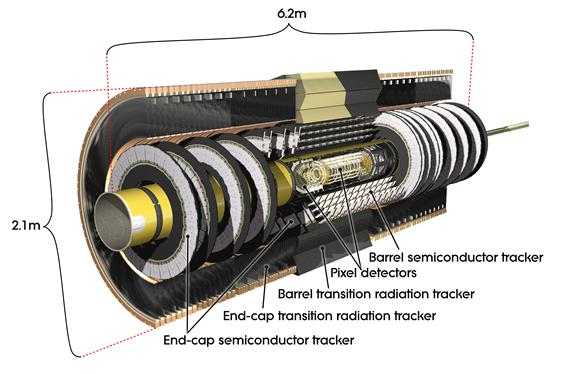
\includegraphics[width=0.7\linewidth]{inner_detector.jpg}
	\caption{A schematic showing the inner detector of the ATLAS detector.~\cite{atlas}}
	\label{fig:lhcandatlas:atlas:inner}
\end{figure}

\begin{itemize}
	\item  \textbf{IBL:} the IBL is an insertable B-layer, placed at the innermost layer of the pixel detector. It was inserted for the LHC Run 2 operation. This layer is composed of silicon pixel modules arranged on carbon fibre staves at a radius of \SI{33}{\milli\meter} surrounding the beam pipe. The IBL provides an additional measurement point closer to the interaction point, and hence improving the impact parameter reconstruction and vertexing.~\cite{ibl}
	
	\item \textbf{Pixel detector:} the pixel detector is a silicon detector, placed at the centre of the ID and has the highest granularity of all the detectors in the ID. The detector is built from 60 million silicon pixels, which have a pixel size of $50\times400$ $\si{\micro\metre^{\text{2}}}$. The high granularity of the pixel detector is used to reconstruct vertices from particle collisions with high resolution. The pixel detector is one of the essential components used to identify jets that have originated from $b$-quarks by precisely reconstructing the primary and secondary vertices.~\cite{atlas}
	
	\item \textbf{SCT:} the SCT is a silicon detector which lies outside the pixel detector around $\SI{300}{\milli\meter}$ away from the beam pipe. It consists of 6 million silicon wafer strip each $\SI{80}{\micro\meter}$ wide, which is designed to track charged particles. It has a track resolution of $\approx\SI{200}{\micro\meter}$, which is not as good as the pixel detector. The SCT has four different layers of modules that are kept around the barrel of the inner detector, and two endcap sections which have nine disks of modules. With the endcap sections, the SCT can provide charged particle tracking up to a pseudorapidity of $|\eta|=2.5$. The SCT contributes to the measurement of 8 different track parameters, including momentum, impact parameter and vertex position.~\cite{atlas}
	
	\item \textbf{TRT:} the TRT is a straw tube detector which covers the largest part of the ID. It provides further tracking information about charged particles. The TRT is made up of straw-tubes which has a diameter of $\SI{4}{\milli\meter}$ which can provide up to 32 hits per track, thus making a considerable contribution to the momentum measurement of the track. The TRT also has some particle identification capabilities through the amount of transition radiation (TR) particle deposits in the detector. TR is the radiation emitted by a relativistic charged particle when it passes through an inhomogeneous medium.~\cite{atlas}
\end{itemize}

%------------------------------------------------------------------------------
\subsubsection{Calorimeters}%
\label{sec:lhcandatlas:atlas:calorimeters}
%------------------------------------------------------------------------------
Calorimeter is used to measure the energy of the particle and identification of the tracks. The ATLAS detector uses two different calorimeter systems, i.e.\ electromagnetic and hadronic calorimeter. These calorimeters measure the deposition of energy from particles. They are sampling calorimeters built from alternating layers of an active material, where the energy measurements are recorded, and an absorbing region, which is used to contain the particles within the calorimeter. The ATLAS calorimeters provide full angular coverage for particles up to $|\eta|<4.9$, but precise energy measurements only for particles with pseudorapidity of $|\eta|<2.5$.~\cite{atlas}

\begin{itemize}
	\item \textbf{Electromagnetic calorimeter:} the electromagnetic calorimeter (ECAL) is used to measure the energy of particles interacting predominantly via electromagnetic interaction with the calorimeter material. These particles include either charged particles that are typically electrons which interact via bremsstrahlung or neutral particles like photons which interacts mainly via electron-positron production. ECAL uses Liquid Argon (LAr) as its active medium, and lead as its absorbing medium. It is divided into three separate regions: the barrel region (covering $|\eta|<1.5$) and two end-cap regions (covering $1.4<|\eta|<3.2$). Since the inner detector only extends to $|\eta|<2.5$, this restricts the precision of measurements in the electromagnetic calorimeter outside this $\eta$ region. This led to the design of the barrel region of the electromagnetic calorimeter having the highest level of granularity.~\cite{atlas} Energy from particles is deposited into four different layers of the electromagnetic calorimeter. The first layer is pre-sampler layer which is placed in front of the electromagnetic calorimeter ($|\eta|<1.8$), and is used to correct for energy loss caused by the ID. Then comes, the first sampling layer which has the highest level of granularity, and is used to provide the very high $\eta-\phi$ resolution required to differentiate between photon and \Pgpz. The second sampling layer is the primary energy deposition layer in the electromagnetic calorimeter. The $\eta-\phi$ resolution of the second layer is around a tenth of the first sampling layer, as the very high $\eta-\phi$ resolution is no longer required. At last, the third sampling layer in which cells are coarser than the other layers of the calorimeter because only very high energy electrons and photons would able to make it to this layer of the electromagnetic calorimeter.~\cite{atlas}
	
	\item \textbf{Hadronic calorimeter:} the hadronic calorimeter (HCAL) is used to measure the energy of particles which interacts predominantly via strong interaction with the calorimeter material, for example, hadrons like protons and neutrons pass through the HCAL, they interact with the nucleus of the material of the HCAL and produce a hadronic shower. HCAL measures the energy deposited by the hadronic shower on the material of the HCAL. It is comprised of five different sections: the barrel tile section ($|\eta|<1.0$), two tile end-cap sections, called the extended barrel ($1.0<|\eta|<1.7$) and two hadronic end-caps ($1.5<|\eta|<3.2$). In the tile regions, thick scintillating plastic panels of \SI{3}{\milli\meter} are used as the active material, and iron plates are used as the absorbing material. These tiles are arranged in a staggered fashion to avoid any gaps within sections of the calorimeter. The scintillation light caused by the tiles is collected by wavelength shifting fibres, which transport the photons to the photomultiplier tubes. The hadronic end-cap calorimeter (HEC) is made from LAr placed between copper absorption layers. LAr acts as an active medium and copper acts as a passive medium. HEC is composed of two disks on either side of the detector. Each disk has 32 modules divided into four different sampling layers.~\cite{atlas}
	
	\item \textbf{Forward calorimeter:} the forward calorimeter (FCAL) is located in the forward region of the ATLAS detector ($3.1<|\eta|<4.9$). It uses LAr as its active material and consists of three parts with different absorption materials. The first part uses copper as a passive material to measure the forward electromagnetic particles. The two other parts are made from Tungsten, which has a very high radiation length and best suited for measuring the forward hadronic particles.~\cite{atlas}
\end{itemize}
 
%------------------------------------------------------------------------------
\subsubsection{Muon spectrometer}%
\label{sec:lhcandatlas:atlas:muonspectrometer}
%------------------------------------------------------------------------------
Muons can pass through the calorimeters without losing much of their energy, so it is difficult to track them. The ATLAS muon spectrometer (MS) is designed to track and measure the \pt of muons originating from the interaction point. An intense magnetic field is required for the muon chambers to be effective over a wide range of \pt and $\eta$. This magnetic field is produced by the toroidal magnetic system which covers the entire muon system.

The muon system consists of two different types of muon chambers: muon drift tubes (MDT) and the cathode-strip chambers (CSC). The muon drift chamber is located in the barrel region of the detector, which provides precise measurements of the location of ionisation tracks from muons passing through the chamber. The most crucial track position is in the primary bending direction of the toroidal magnetic field, as this direction is used to calculate the curvature of the muon track, and hence the \pt of the muon. The cathode-strip chambers are located in the forward region of the ATLAS detector and are designed to handle a high occupancy of low \pt forward muons. The CSCs are multiwire proportional chambers, where the wires are oriented in the radial direction pointing to the centre of the muon CSC wheel. Resistive plate chambers (RPCs) are used to trigger on muons in the barrel section, and thin gap chambers (TGCs) are used to trigger on muons in the end-cap sections.~\cite{atlas}

%------------------------------------------------------------------------------
\subsubsection{Magnets}%
\label{sec:lhcandatlas:atlas:magnets}
%------------------------------------------------------------------------------
The ATLAS detector uses two different magnet systems to measure the momentum of the charged particles accurately. The first magnet system is a solenoid magnet which provides an axial magnetic field of \SI{2}{\tesla}. It covers the whole inner detector. The second magnetic system is toroidal, which produces magnetic fields in the muon system. It is divided into two parts: barrel region which is located around the central calorimeter and the end-caps which are situated at the two ends of the detector. The magnetic field strength in the barrel region is \SI{0.5}{\tesla} which increases to \SI{1}{\tesla} in the end cap regions of the muon system.~\cite{atlas}

%------------------------------------------------------------------------------
\subsubsection{Trigger system}%
\label{sec:lhcandatlas:atlas:trigger}
%------------------------------------------------------------------------------
Due to the high luminosity of the LHC in Run 2, a large storage system is required to store the information about every event. There are a lot of events which are not interesting for the physics analysis for various reasons. So, the ATLAS detector needs a trigger system to only select and store those events which are interesting for the physics analysis. The ATLAS trigger system is divided into two parts: Level-1 trigger and the High-Level trigger (HLT). Level-1 is entirely a hardware-based trigger and is constructed from specialised electronics. It uses the raw information from the muon systems and calorimeters to search for high energy physics objects, such as jets, electrons, photons, muons and decayed taus. The HLT is an event filter which includes processing of the data using the full detector information. Events that pass the Level-1 trigger are reduced to the event rate of \SI{100}{\kilo\hertz} from \SI{40}{\mega\hertz}. Then, they are passed to the HLT, which further reduces the event rate to \SI{1}{\kilo\hertz}.~\cite{atlas}


%%% Local Variables: 
%%% mode: latex
%%% TeX-master: "mythesis"
%%% End: 
